%%%%%%%%%%%%%%%%%%%%%%%%%%%%%%%%%%%%%%%%%%%%%%%%%%%%%%%%%%%
\section{Preliminars}
%%%%%%%%%%%%%%%%%%%%%%%%%%%%%%%%%%%%%%%%%%%%%%%%%%%%%%%%%%%
%
%
%%%%%%%%%%%%%%%%%%%%%%%%%%%%%%%%%%%%%%%%%%%%%%%%%%%%%%%%%%%
\subsection{Research question}
%%%%%%%%%%%%%%%%%%%%%%%%%%%%%%%%%%%%%%%%%%%%%%%%%%%%%%%%%%%
%
%
\begin{frame}[t, negative]
	\subsectionpage
\end{frame}
%
%
\begin{frame}
	{Research question}
	%
	On two fronts:
	%
	\begin{enumerate}
		%
		\item Can comparative judgement \textcolor{blue}{(CJ)} methods be used to assess speech intelligibility \textcolor{blue}{(SI)}?, \\
		To investigate this wee need:
		%
		\begin{itemize}
			\item an \alert{objective measure} of SI
		\end{itemize}
		%
		%
		\item where CJ stands versus absolute holistic judgement \textcolor{blue}{(HJ)} methods?, \\ 
		In terms of:
		%
		\begin{itemize}
			\item validity
			\item reliability
			\item statistical efficiency
			\item time efficiency
		\end{itemize}
		%
	\end{enumerate}
	%
\end{frame}
%
%
\begin{frame}
	{Objective measure of SI}
	%
	the \alert{most objective} measure of SI (we know of) comes from a \textcolor{blue}{transcription task}:
	
	\begin{enumerate}
		%
		\item transcribing children's utterances (made by multiple judges),
		%
		\item align transcriptions at the utterance level,
		%
		\item calculate an entropy measure (H), defined as
		%
		\begin{equation*} \label{eq:entropy}
			H = H(\pmb{p}) = \frac{-\sum_{i=1}^{n} p_{i} \cdot \log_{2}(p_{i})}{\log_{2}(N)}
		\end{equation*}
		%
		\item characteristics of $H$ \citep{Boonen_et_al_2021, Faes_et_al_2021} 
		%
		\begin{itemize}
			\item  bounded in $[0,1]$ space,
			%
			\item utterances with more agreement are more intelligible, and therefore $H \rightarrow 0$,
			%
			\item utterances with low agreement are less intelligible, and therefore $H \rightarrow 1$.
		\end{itemize}
		%
	\end{enumerate}
	%
\end{frame}
%
%
%%%%%%%%%%%%%%%%%%%%%%%%%%%%%%%%%%%%%%%%%%%%%%%%%%%%%%%%%%%
\subsection{Research hypothesis production}
%%%%%%%%%%%%%%%%%%%%%%%%%%%%%%%%%%%%%%%%%%%%%%%%%%%%%%%%%%%
%
%
\begin{frame}[t, negative]
	\subsectionpage
\end{frame}
%
%
\begin{frame}
	{A typical scientific lab\footnote{\citet{McElreath_2020}, lecture $20$ and \citet{McElreath_2022}, chapter $17$}}
	%
	\begin{columns}
		%
		\begin{column}{0.5\textwidth}
			%
			What is needed?
		
			\begin{enumerate}
				%
				\item Quality of theory
				\item Quality of data
				\item Reliable procedures and code
				\item Quality of data analysis
				\item Documentation
				\item Reporting
				%
			\end{enumerate} 
			%
		\end{column}
		%
		\begin{column}{0.5\textwidth}  
			%
			What we will deal with:
			%
			\begin{enumerate}
				%
				\item \textcolor{blue}{Quality of theory}
				\item \textcolor{blue}{Quality of data}
				\item \alert{Reliable procedures and code}
				\item \textcolor{blue}{Quality of data analysis}
				\item \textcolor{blue}{Documentation}
				\item Reporting
				%
			\end{enumerate} 
			%
		\end{column}
		%
	\end{columns}
	%
\end{frame}
%
%
\begin{frame}
	{Research hypothesis production\footnote{\citet{Hernan_2020}, lesson $4$}}
	%
	\begin{columns}
		%
		\begin{column}{0.5\textwidth}
			%
			Well known challenges
			%
			\begin{itemize}
				%
				\item Insufficient data
				\item Wrong population
				\item Measurement error
				\item Selection bias
				\item Confounding
				%
			\end{itemize} 
			%
		\end{column}
		%
		\begin{column}{0.5\textwidth} 
			% 
			Known challenges in our research;
			%
			\begin{itemize}
				%
				\item \textcolor{blue}{Insufficient data (possibly)}
				\item Wrong population
				\item \textcolor{blue}{Measurement error}
				\item \textcolor{blue}{Selection bias}
				\item \textcolor{blue}{Confounding}
				%
			\end{itemize} 
			%
		\end{column}
		%
	\end{columns}
	%
\end{frame}
%
%
\begin{lhframe}[rhgraphic={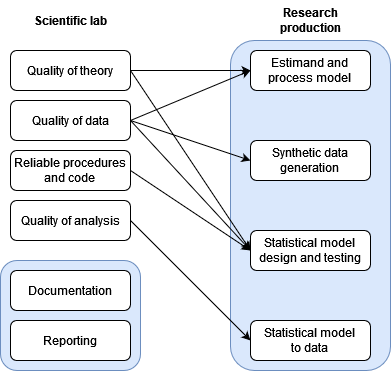
\includegraphics[scale=0.43]{lab_to_research.png}}]
	{Research hypothesis schematics\footnote{\citet{McElreath_2022}, lecture $20$, \citet{Pearl_2019}. Follow \citet{Fogarty_et_al_2022} on item (c).}}
	
	\begin{enumerate}
		%
		\item[a.] Estimand and \textcolor{blue}{process model}
		\item[b.] Synthetic data generation
		\item[c.] Statistical model design and testing
		\item[d.] Apply \textcolor{blue}{statistical model} to data 
		%
	\end{enumerate} 
	%
\end{lhframe}
%
%
\begin{lhframe}[rhgraphic={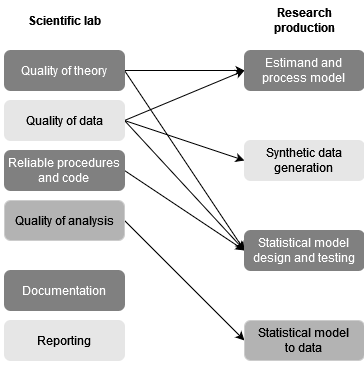
\includegraphics[scale=0.60]{DAG_to_research.png}}]
	{Why do we need to follow this?}
	
	Because the improvement of:
	%
	\begin{itemize}
		%
		\item A clear definition of the estimand and process model (assumptions).
		%
		\item An improved the reliability of your procedures.
		%
		\item As a documentation procedure.
		%
	\end{itemize}
	
	leads to:
	%
	\begin{itemize}
		%
		\item A sound analysis, and sound results \alert{(even when we cannot answer our question)}.
		%
		\item An improved planning to get data.
		%
	\end{itemize}
	%
\end{lhframe}
%
%